\textbf{Obtener el nombre de todos los clientes que vivan en la región West y hayan solicitados productos de las categorías Technology o Furniture. El pedido debió de solicitarse en 2106 y el modo de envío debe ser Standard Class.}

Asumiré que cuando dice "El pedido debió de solicitarse en 2106" se refiere al 2016. 

\begin{center}
    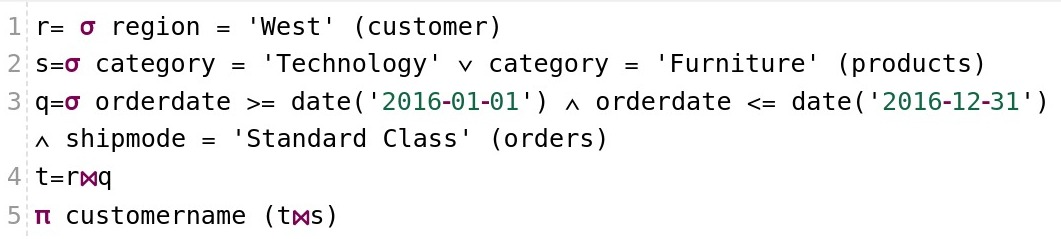
\includegraphics[width=5cm]{resources/pregunta2/2.3.1}
\end{center}
Para esta consulta 
\begin{itemize}
    \item \textbf{r} es la tabla de clientes de la región West
    \item \textbf{s} es la tabla de productos de categoría Technology o Furniture
    \item \textbf{q} es la tabla de pedidos enviados en modo Standard Class en el 2016
    \item \textbf{t} es la relacion de clientes que viven en West que hicieron un pedido en modo Standard Class en el 2016
    \item \textbf{t join s} es la relacion de clientes que viven en West que hicieron un pedido en modo Standard Class en el 2016, y ademas su producto es de categoria Technology o Furniture
\end{itemize}

El resultado es:
\begin{center}
    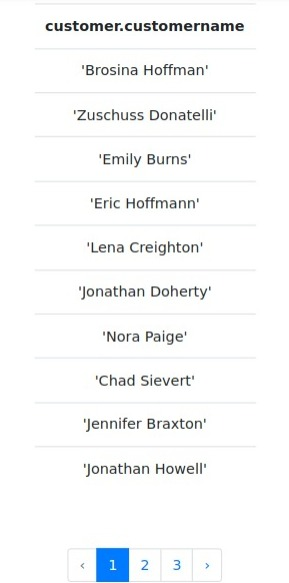
\includegraphics[width=5cm]{resources/pregunta2/2.3.2}
\end{center}

Nótese que primero hacemos join de r con q, ya que el atributo en común es customerid, de otra forma obtendríamos el producto cartesiano, lo cuál es demasiado costoso en términos de recursos. 
\begin{center}
    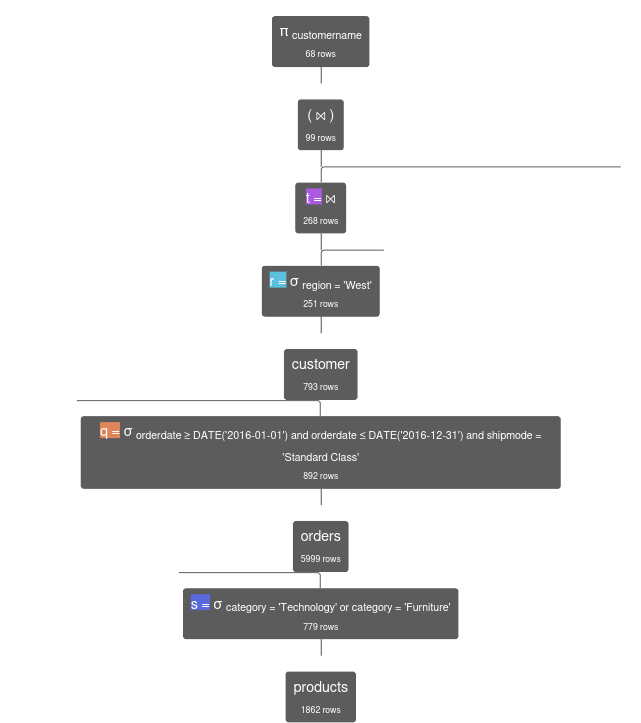
\includegraphics[width=5cm]{resources/pregunta2/2.3.3}
\end{center}
